\chapter{Resultados Preliminares}
\label{chap:resultados}
Para alcançar o objetivo final deste trabalho, fez-se uma modularização do problema que será validada e integrada, módulo a módulo. Para a primeira parte do trabalho, supõe-se que o robô já tenha encontrado o alvo e precisa simplesmente circular ao seu redor. Ou seja, precisa realizar um movimento circular uniforme. Para tal, foi necessário elaborar a malha de controle 1 que é responsável pelo controle de velocidade de cada roda. 

Sendo assim, foi estabelecido o raio (\emph{R}) e o período (\emph{T}) em que o robô pretende circular ao redor do alvo. Definindo-se \emph{R} igual a $15cm$ e $T = 5s$. Tem-se que a velocidade angular desejada do robô ($\omega_{d}$) será de $1,256 rad/s$, conforme \autoref{eq:velocangular}. E a velocidade linear desejada ($v_{d}$) do robô será de $0,1884 m/s$, supondo o ideal que é um sistema já estabilizado. Ou seja, em movimento circular uniforme onde tem-se que: 

\begin{equation}
v = \omega R 
\label{eq:veloclinear}
\end{equation}

A partir destas definições foram utilizados os \emph{encoders} do próprio \emph{Lego Mindstorms} para obter a velocidade real ($\omega_{rr},\omega_{rl}$) de cada roda e as equações \ref{eq:velocangulardireita} e \ref{eq:velocangularesquerda}, para calcular a velocidade angular desejada de cada roda ($\omega_{dr},\omega_{dl}$), para que o robô entre em movimento circular uniforme. E assim, foram utilizadas as equações \ref*{eq:errVelAngDireita} e \ref*{eq:errVelAngEsquerda}, para o cálculo do erro da velocidade angular ($e_{wr},e_{wl}$). Este erro alimenta o controlador que retorna como saída, a potência ($pwm_{r}, pwm_{l}$) que será passada a cada motor.

Foram implementados três tipos de controladores diferentes, afim de comparar o desempenho dos mesmos para resolução do problema. Primeiro, implementou-se um controlador simples que acresce de uma unidade a potência do motor quando a um erro maior que zero, ou decresce, caso haja um erro menor que zero. É importante ressaltar que os motores do \emph{kit Lego Mindstorms} aceitam comandos de potência que variam de $-100$ a $100$. Logo, poderiam haver situações em que a potência passada aos motores excederia aos limites do motor, para evitar a saturação dos atuadores, foi definido um limite para a saída do controlador que respeite às limitações da plataforma.

Ao utilizar a ferramenta \emph{MATLAB} para visualizar o erro de velocidade angular, percebe-se que ela converge para zero como esperado, como mostrado na \autoref{fig:ewdc}.

\begin{figure}[!htb]
	\centering
	\caption{Erro de velocidade angular - Controle Simples}
	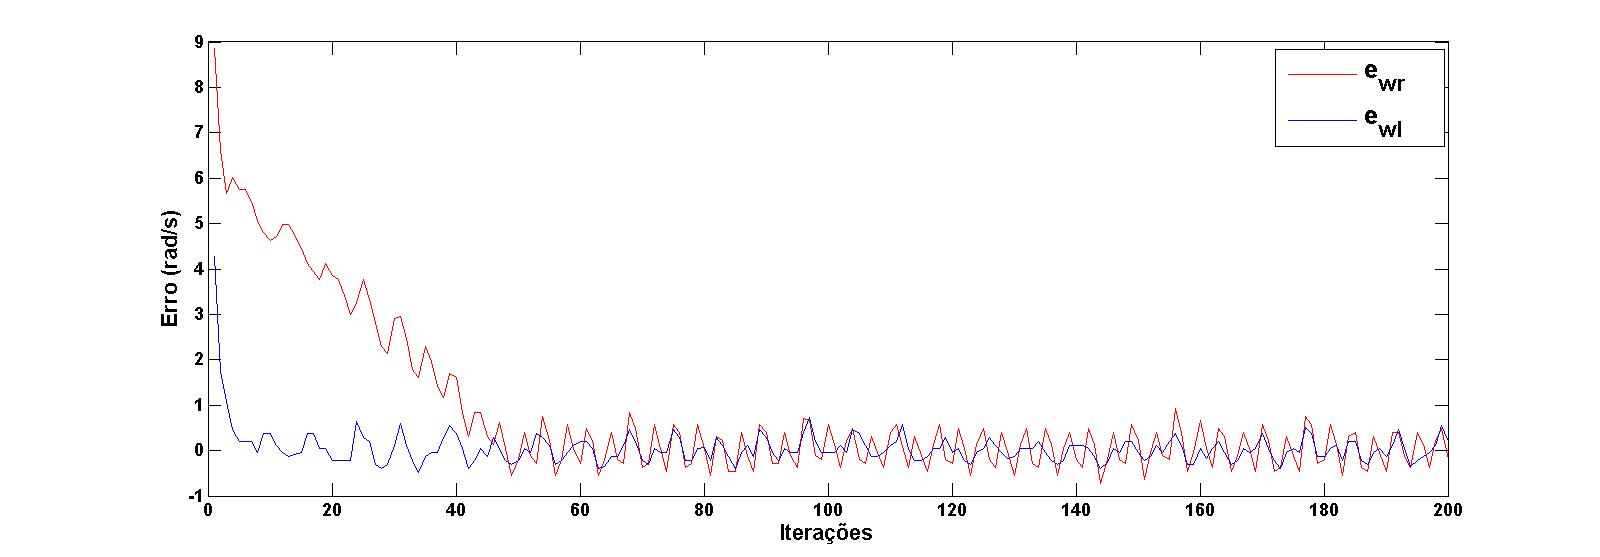
\includegraphics[width=1.0\textwidth]{./04-figuras/Ewd_b1c}
	\
	\label{fig:ewdc}
\end{figure}

Entretanto, ao observar a trajetória do robô no plano e ao plotar no \emph{MATLAB} a trajetória do mesmo,utilizando-se as equações \ref*{eq:posiçãoxreal}, \ref*{eq:posiçãoyreal} e \ref*{eq:posiçãothetareal}, percebe-se que ele demora um pouco para realizar o movimento circular, como demonstrado na \autoref{fig:trajc}.

\begin{figure}[!htb]
	\centering
	\caption{Trajetória do Robô (R: $15cm$) - Controle Simples}
	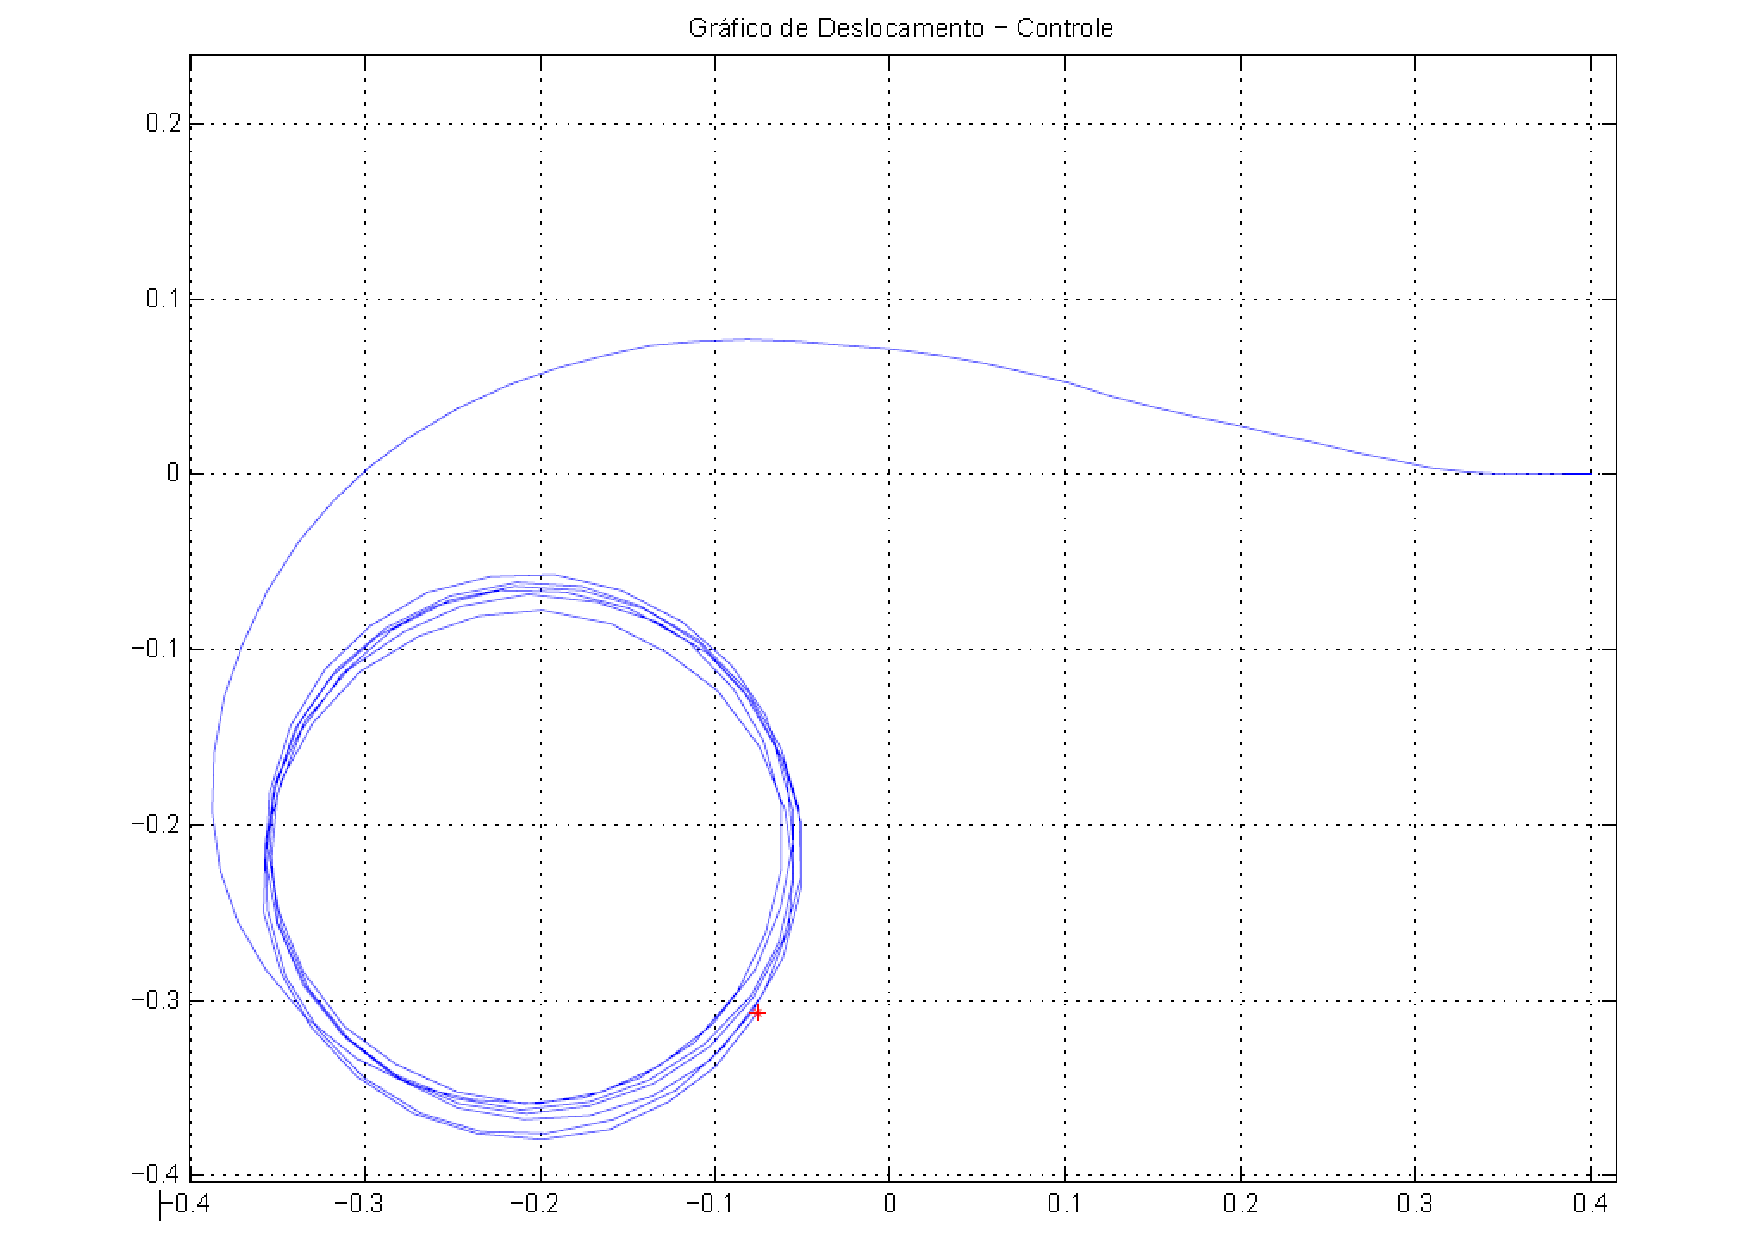
\includegraphics[width=1.0\textwidth]{./04-figuras/trajetoria_b1_15_c}
	\
	\label{fig:trajc}
\end{figure}

Feito isso, para fins de comparação, implementou-se um controlador PI, de ganho proporcional ($k_{p}$) igual a 10 e ganho integral ($k_{i}$) igual a 1 e obteve-se os erros e a trajetória demonstrados pelas figuras \ref*{fig:ewd_pi_15} e \ref*{fig:traj_pi_15}. 

\begin{figure}[!htb]
	\centering
	\caption{Erro de velocidade angular - Controle PI: $k_{p}=10,k_{i}=1$ - Raio 15cm}
	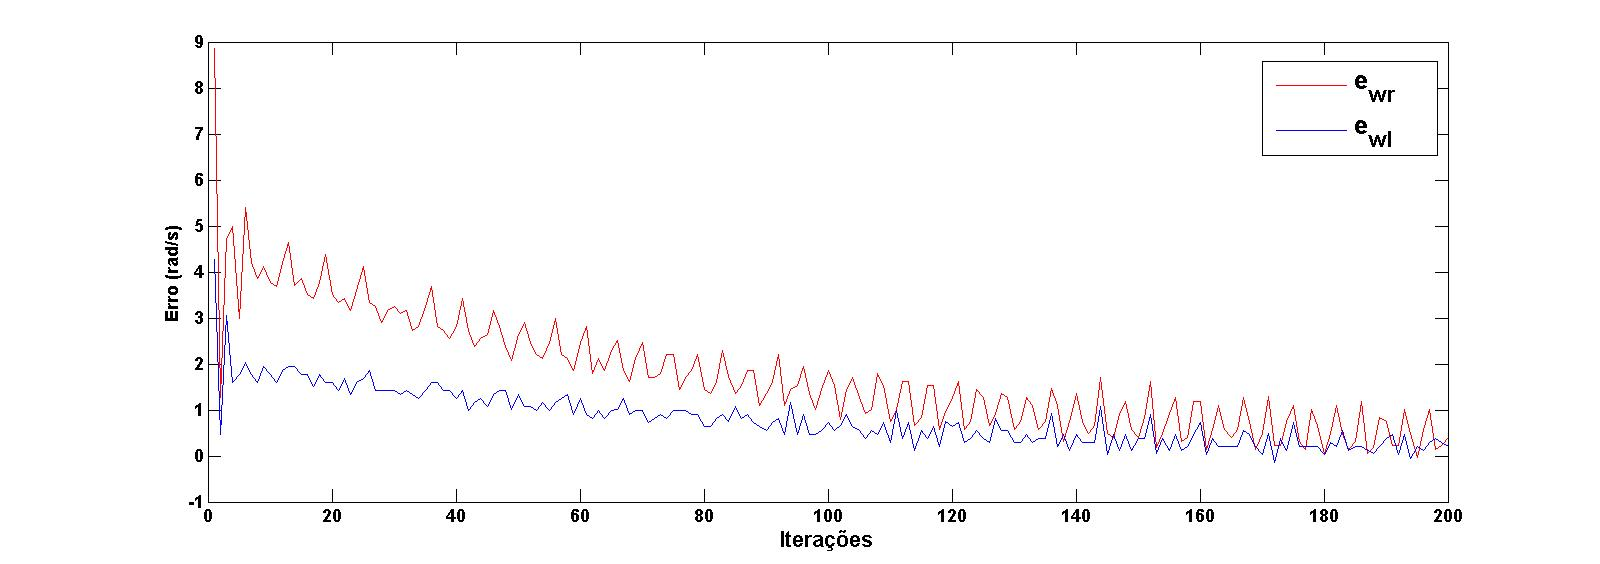
\includegraphics[width=1.0\textwidth]{./04-figuras/Ewd_b1_pi_15}
	\
	\label{fig:ewd_pi_15}
\end{figure}

\begin{figure}[!htb]
	\centering
	\caption{Trajetória do Robô (R: $15cm$) - Controle PI: $k_{p}=10,k_{i}=1$}
	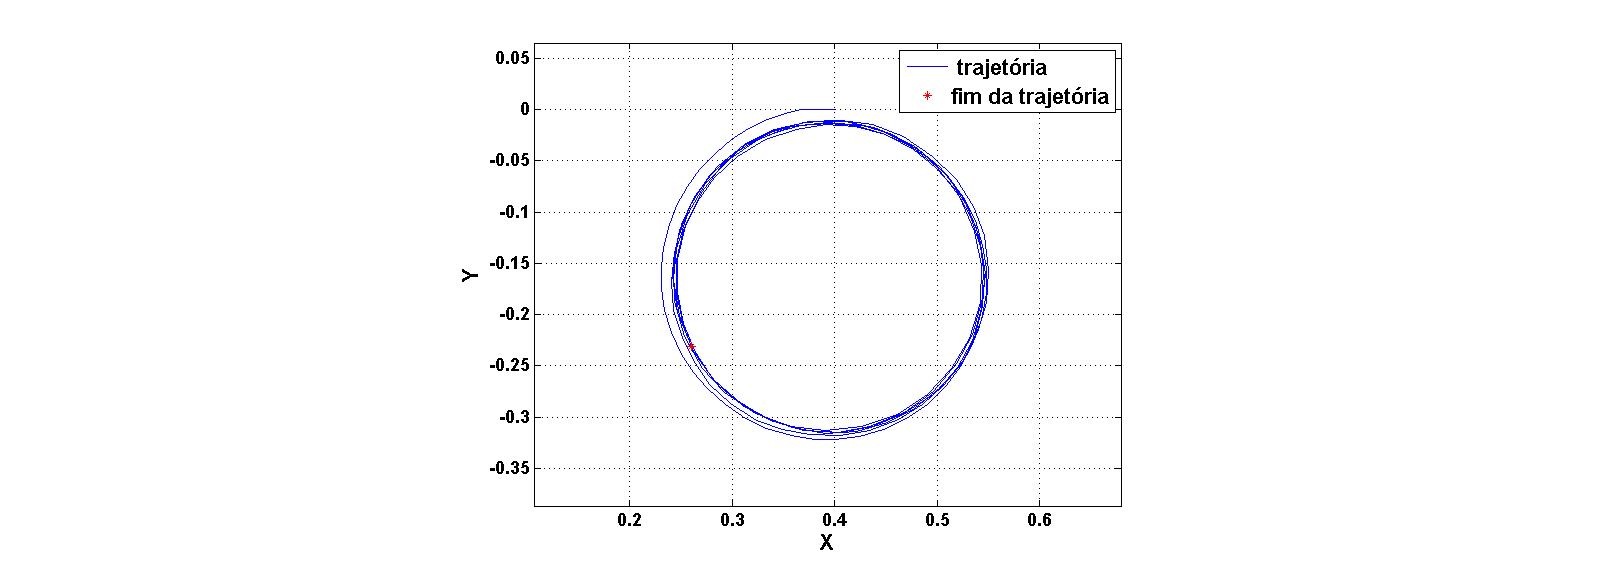
\includegraphics[width=1.0\textwidth]{./04-figuras/trajetoria_b1_15_pi}
	\label{fig:traj_pi_15}
\end{figure}

Observando as figuras \ref{fig:ewdc} e \ref{fig:ewd_pi_15} é possível notar que ambos os controladores tendem à diminuir o erro de velocidade. Contudo, ao verificar na figura comparativa \autoref{fig:err_comparativo1} é possível perceber que o controlador simples converge mais rapidamente que o controlador \emph{PI}. Entretanto, embora  o controlador simples convirja mais rapidamente, o que se mostra no comparativo da trajetória (\autoref{fig:traj_comparativo1}) de ambos os controladores, é que o controlador \emph{PI}, converge mais rapidamente para a trajetória desejada. Sendo assim, foram realizados mais experimentos com variações do controlador \emph{PI}, como será visto a seguir. 

\begin{figure}[!htb]
	\centering
	\caption{Comparativo - Erro de velocidade angular - Controle PI e Controle Simples - Raio 15cm}
	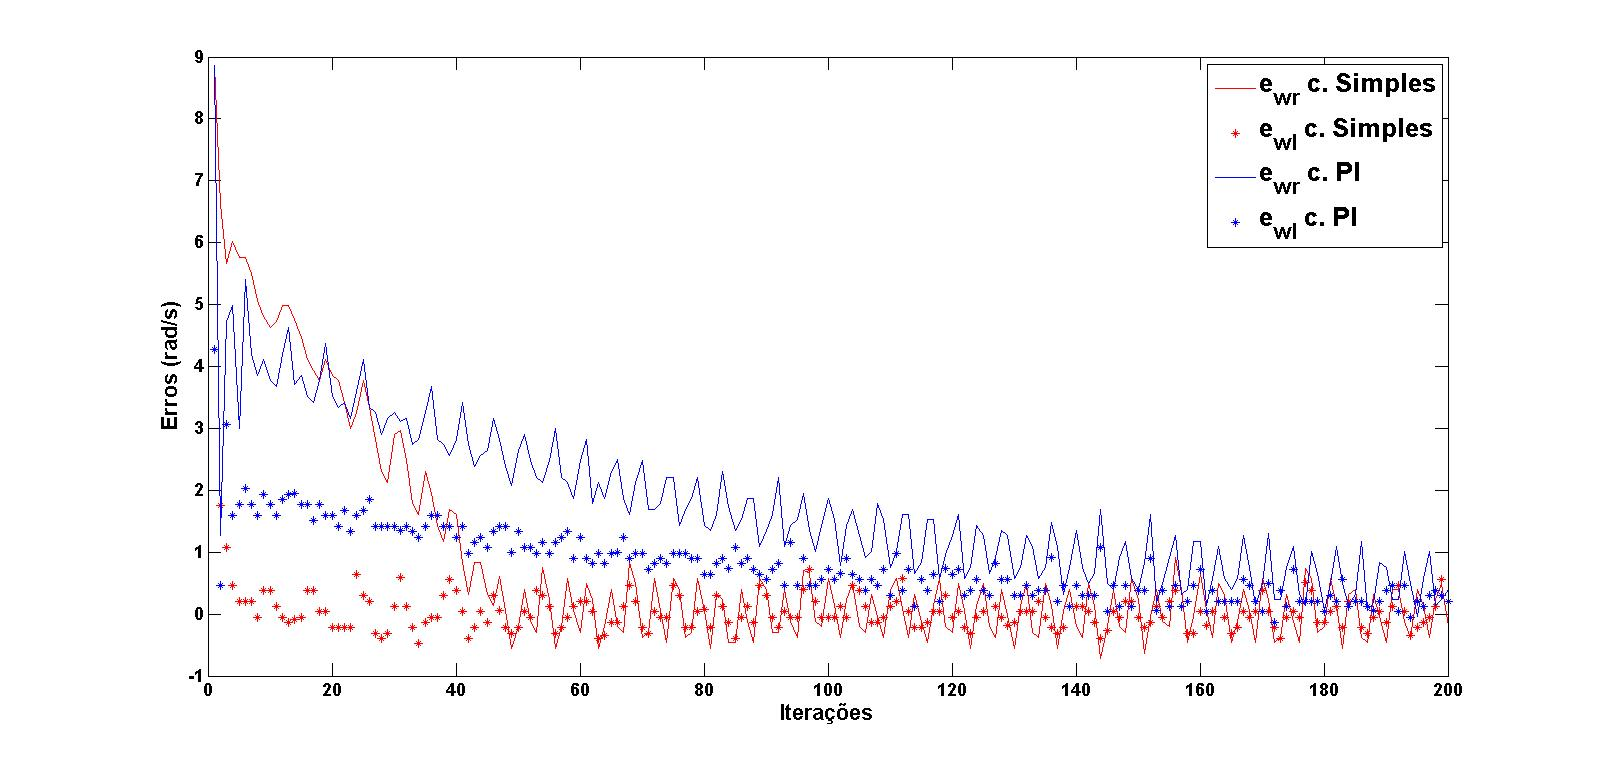
\includegraphics[width=1.0\textwidth]{./04-figuras/ew_comparativo1}
	\
	\label{fig:err_comparativo1}
\end{figure}

\begin{figure}[!htb]
	\centering
	\caption{Comparativo da Trajetória do Robô (R: $15cm$) - Controle PI e Controle Simples}
	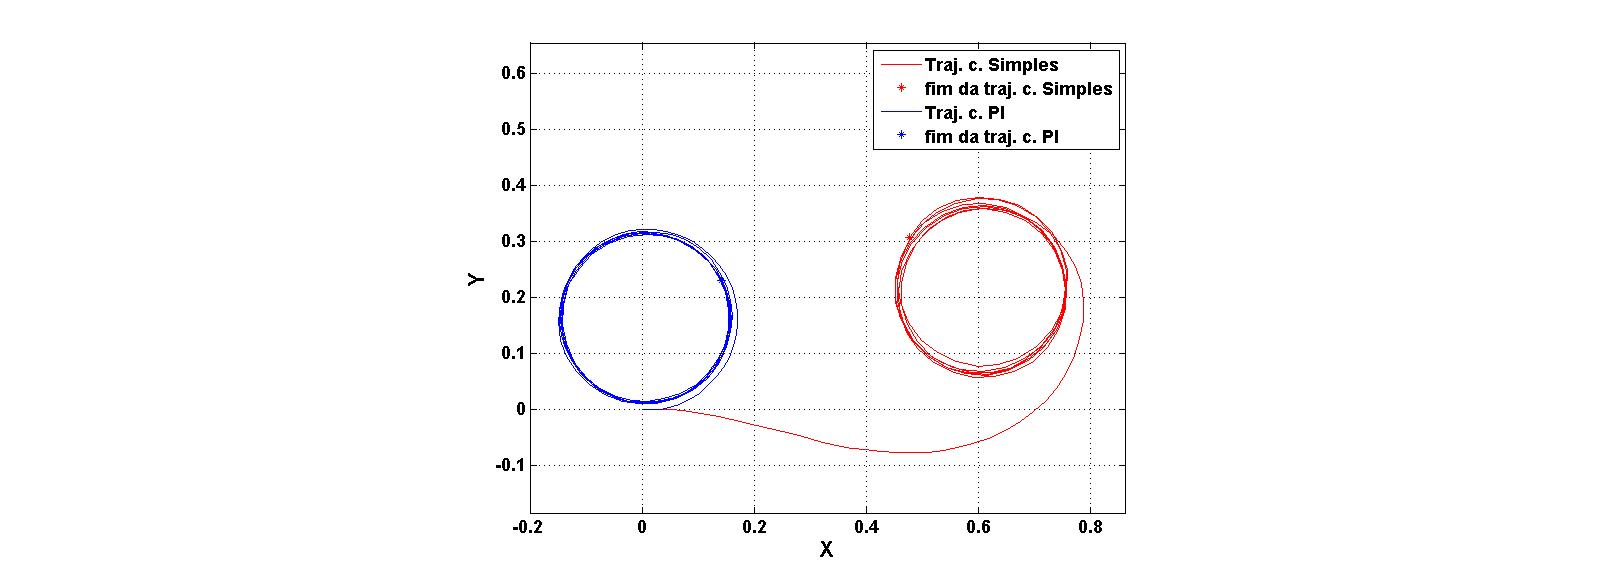
\includegraphics[width=1.0\textwidth]{./04-figuras/traj_comparativo1}
	\label{fig:traj_comparativo1}
\end{figure}

Primeiro, fez-se testes variando o ganho proporcional ($k_{p}$). Notou-se, como comprovado pela \autoref{fig:pi_inst} que ao dobrar $k_{p}$, o sistema se tornava instável, como previsto na \autoref{sec:pid}, que indica que quanto maior o ganho, mais o sistema tende à se instabilizar. Depois, foi realizada uma comparação, alterando-se os parâmetros de $k_{p}$ e $k_{i}$, como mostrado na \autoref{fig:comparaivoPI}. E por fim, foram realizados experimentos variando o raio do perímetro ao redor do alvo, como exemplificado na \autoref{fig:traj_pid_30}, onde observa-se que a trajetória é suficientemente precisa, conforme o sistema se estabiliza. 
\begin{figure}[!htb]
	\centering
	\caption{Erro de velocidade angular - Controle PI: Sistema Instável - Raio 15cm}
	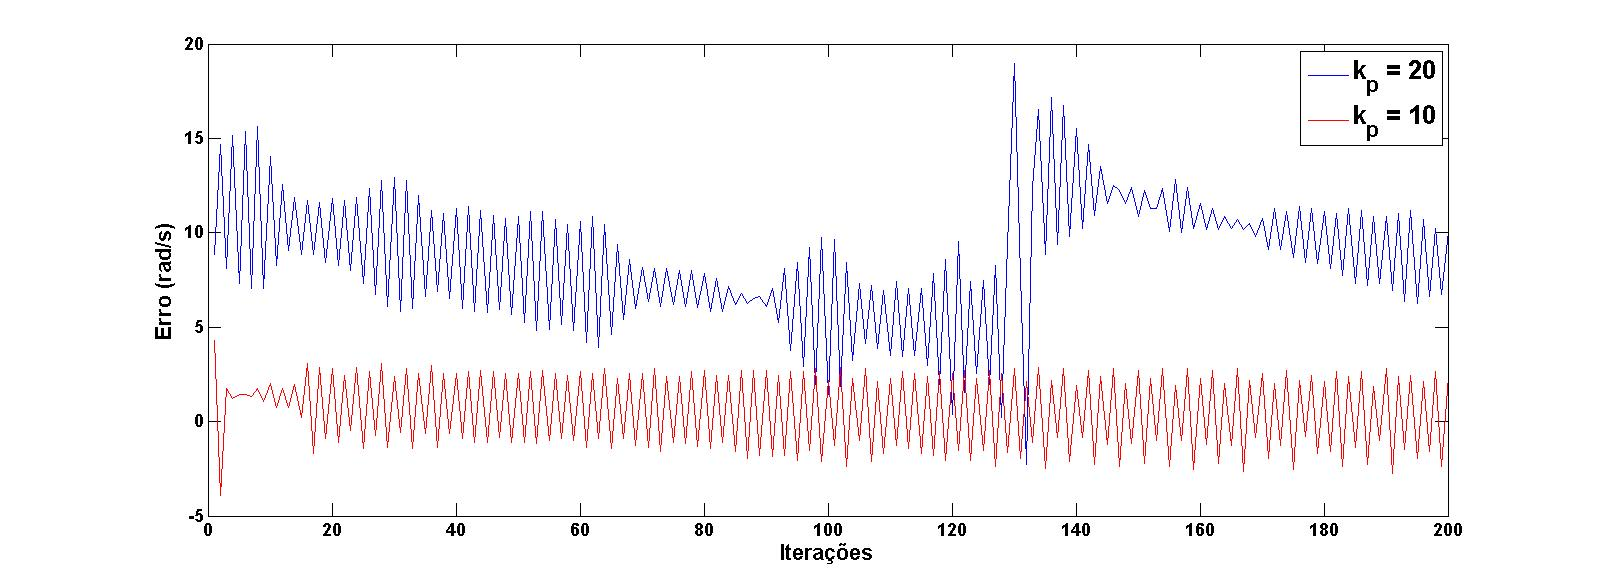
\includegraphics[width=1.0\textwidth]{./04-figuras/pi_inst}
	\
	\label{fig:pi_inst}
\end{figure}
\begin{figure}[!htb]
	\centering
	\caption{Comparativo: Erro de velocidade angular - Controladores PI}
	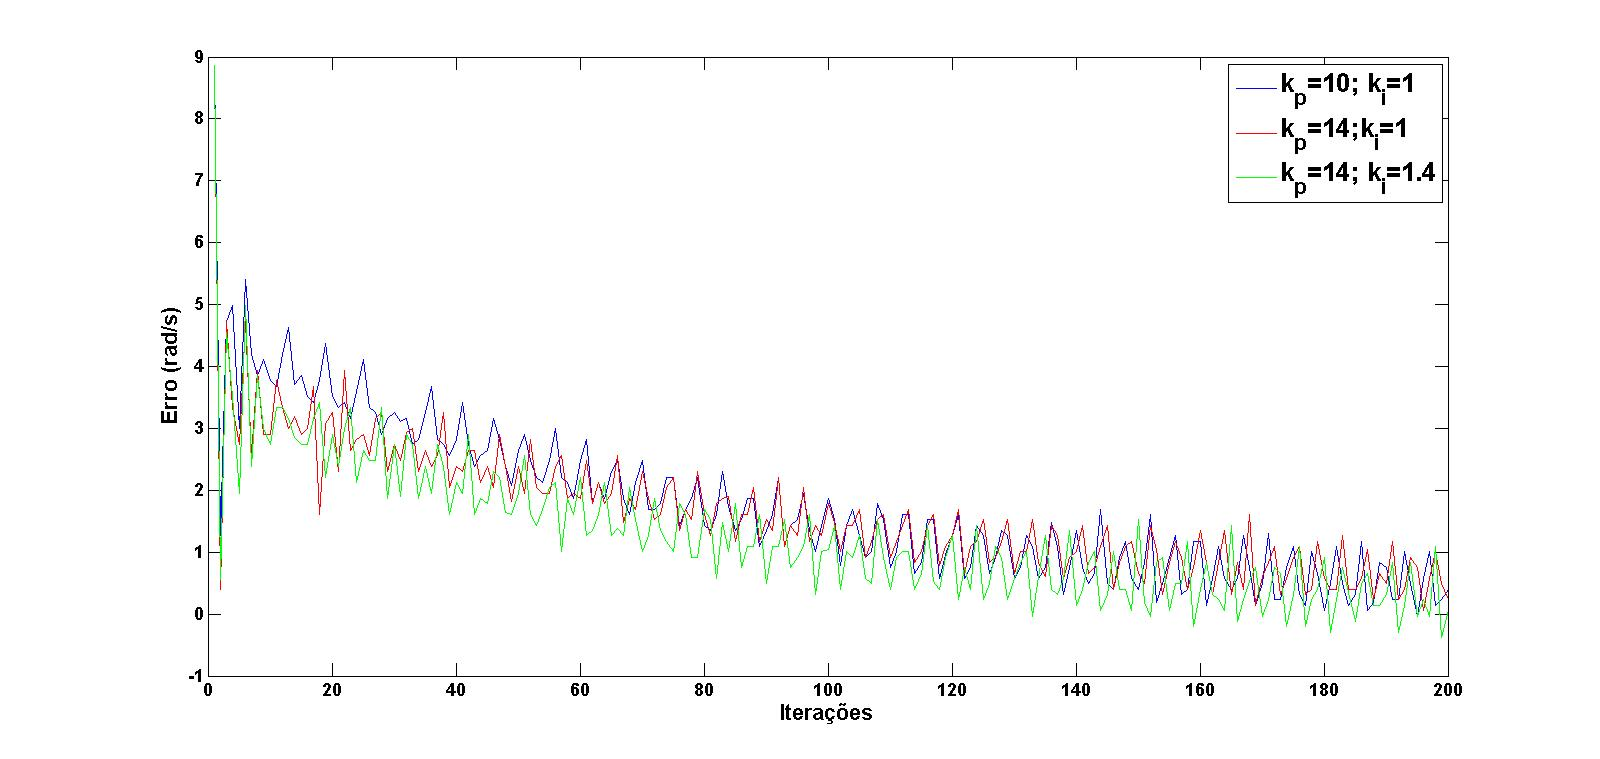
\includegraphics[width=1.0\textwidth]{./04-figuras/comparativoPI}
	\
	\label{fig:pi_inst}
\end{figure}

\begin{figure}[!htb]
	\centering
	\caption{Trajetória do Controladores PID - Raio $30cm$}
	\includegraphics[width=1.0\textwidth]{./04-figuras/trajetória_pid_30}
	\
	\label{fig:traj_pid_30}
	\end{figure}

